%%%%%%%%%%%%%%%%%%%%%%%%%%%%%%%%%%%%%%%%%
% University/School Laboratory Report
% LaTeX Template
% Version 3.1 (25/3/14)
%
% This template has been downloaded from:
% http://www.LaTeXTemplates.com
%
% Original author:
% Linux and Unix Users Group at Virginia Tech Wiki 
% (https://vtluug.org/wiki/Example_LaTeX_chem_lab_report)
%
% License:
% CC BY-NC-SA 3.0 (http://creativecommons.org/licenses/by-nc-sa/3.0/)
%
%%%%%%%%%%%%%%%%%%%%%%%%%%%%%%%%%%%%%%%%%

%----------------------------------------------------------------------------------------
%	PACKAGES AND DOCUMENT CONFIGURATIONS
%----------------------------------------------------------------------------------------

\documentclass{article}

\usepackage[version=3]{mhchem} % Package for chemical equation typesetting
\usepackage{siunitx} % Provides the \SI{}{} and \si{} command for typesetting SI units
\usepackage{graphicx} % Required for the inclusion of images
\usepackage{natbib} % Required to change bibliography style to APA
\usepackage{amsmath} % Required for some math elements 
\usepackage[margin=1in]{geometry}
\usepackage{hyperref}
\usepackage[british]{babel}
\selectlanguage{british}


\setlength\parindent{0pt} % Removes all indentation from paragraphs

\renewcommand{\labelenumi}{\alph{enumi}.} % Make numbering in the enumerate environment by letter rather than number (e.g. section 6)

%\usepackage{times} % Uncomment to use the Times New Roman font

%----------------------------------------------------------------------------------------
%	DOCUMENT INFORMATION
%----------------------------------------------------------------------------------------

\title{Computer Vision - Lab 5 \\ Panoramic Image} % Title

\author{Davide Dravindran Pistilli} % Author name

\date{\today} % Date for the report

\begin{document}

\maketitle % Insert the title, author and date

\section{Introduction}
The purpose of this lab experience is the creation of a panoramic image from a set of consecutive pictures.
In order to run, the program requires the following command line arguments:
\begin{itemize}
\item \textbf{Image folder}: the folder where the source images are stored.
\item \textbf{Image field of view}: the field of view of the images, it must be the same for all of them.
\item \textbf{Distance ratio}: larger values allow for higher error margins.
\end{itemize}

\section{Workflow}
The first step is to perform a cylindrical projection of all source images. After each projection, the corresponding histograms are equalised on order to improve results.
After this pre-processing step is performed, the keypoints and descriptors for each image are computed. The algorithm can use either ORB or SIFT features in order to compare the two results.
Using the features from the previous step, matches are computed between each consecutive pair of images. In order to avoid bad matches, the \textit{distance ratio} parameter is used to remove those based on really different keypoints.
Furthermore, a homography matrix is computed between the two images. This allows to further improve the quality of the matches by removing all outliers that don't fit the transformation.
At this point the average translation between matches can be computed.

The actual panoramic image is computed considering both horizontal and vertical translations that were computed before. Since the border between images is usually quite visible, a Gaussian blur with a (1, 7) kernel and $\sigma=2.5$ is applied to all transitions.

No final histogram equalisation was applied, since it only worsened the result.

\section{Results}
The program was tested on 5 different datasets with both ORB and SIFT features in order to compare their results.
The best parameters are:\\

\begin{center}
\begin{tabular}{ |c|c|c| }
\hline
Dataset & Ratio & Features \\
\hline
\hline
Dolomites & 2.5 & both \\
\hline
Kitchen & 2.5 & both \\
\hline
Lab & 6.0 & both \\
\hline
Lab automatic & 2.5 & SIFT \\
\hline
Lab manual & 2.5 & SIFT \\
\hline
\end{tabular}
\end{center}

While in the Kitchen dataset both ORB and SIFT performed similarly, in all the others SIFT proved to identify better features.
Both in the Dolomites and in the Lab datasets, in fact, SIFT tolerated larger changes to the ratio than ORB. Furthermore, in the last two datasets ORB did not provide a correct result, irrespective of the chosen ratio.
Some example outputs are provided below.

\begin{figure}[h]
\begin{center}
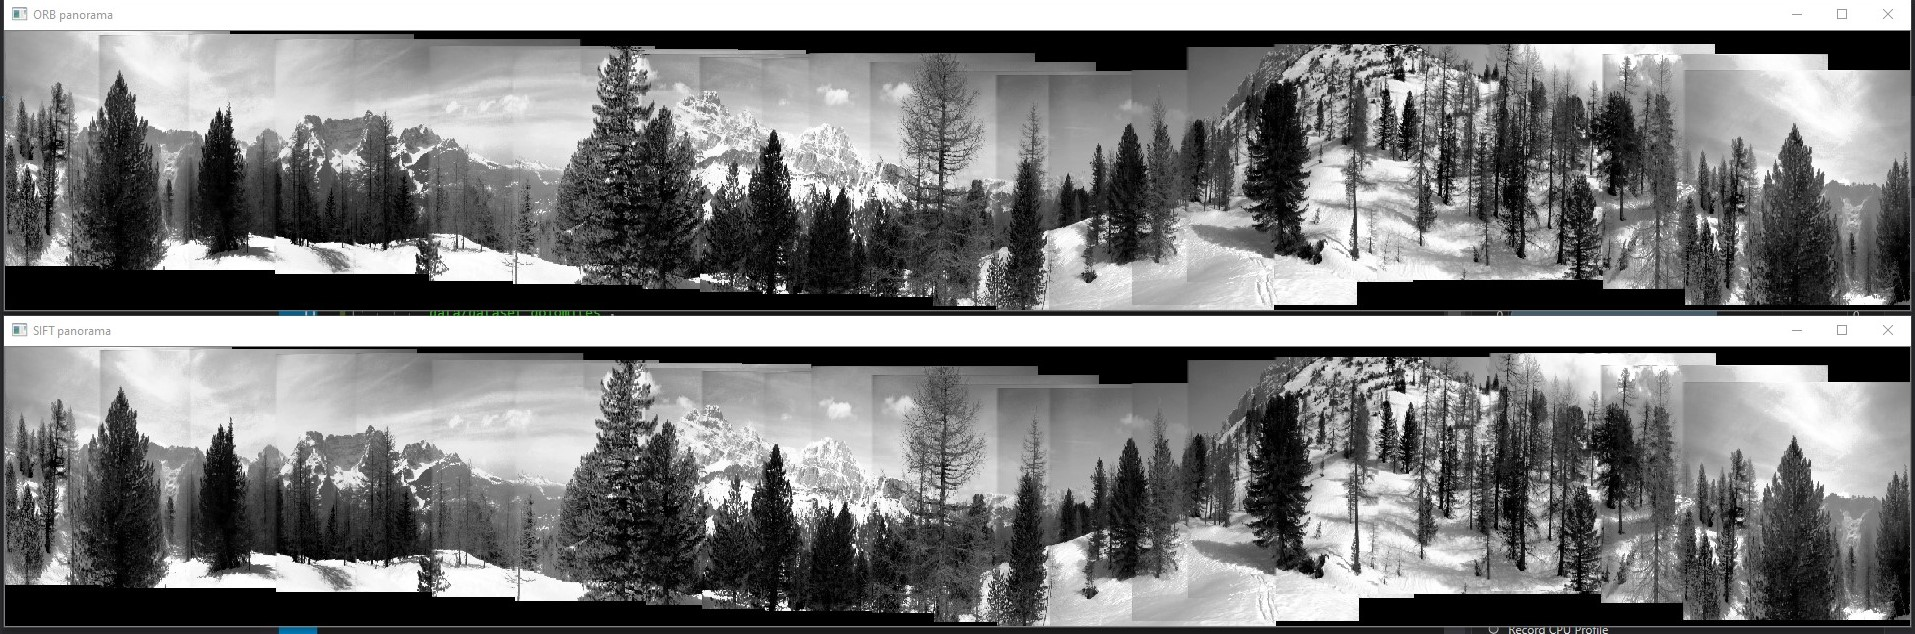
\includegraphics[width=1\textwidth]{images/dolomites}
\caption{\footnotesize{in the Dolomites dataset we can see a high vertical translation, which got correctly fixed by both ORB and SIFT.}}
\label{img_dolomites}
\end{center}
\end{figure}

\begin{figure}[h]
\begin{center}
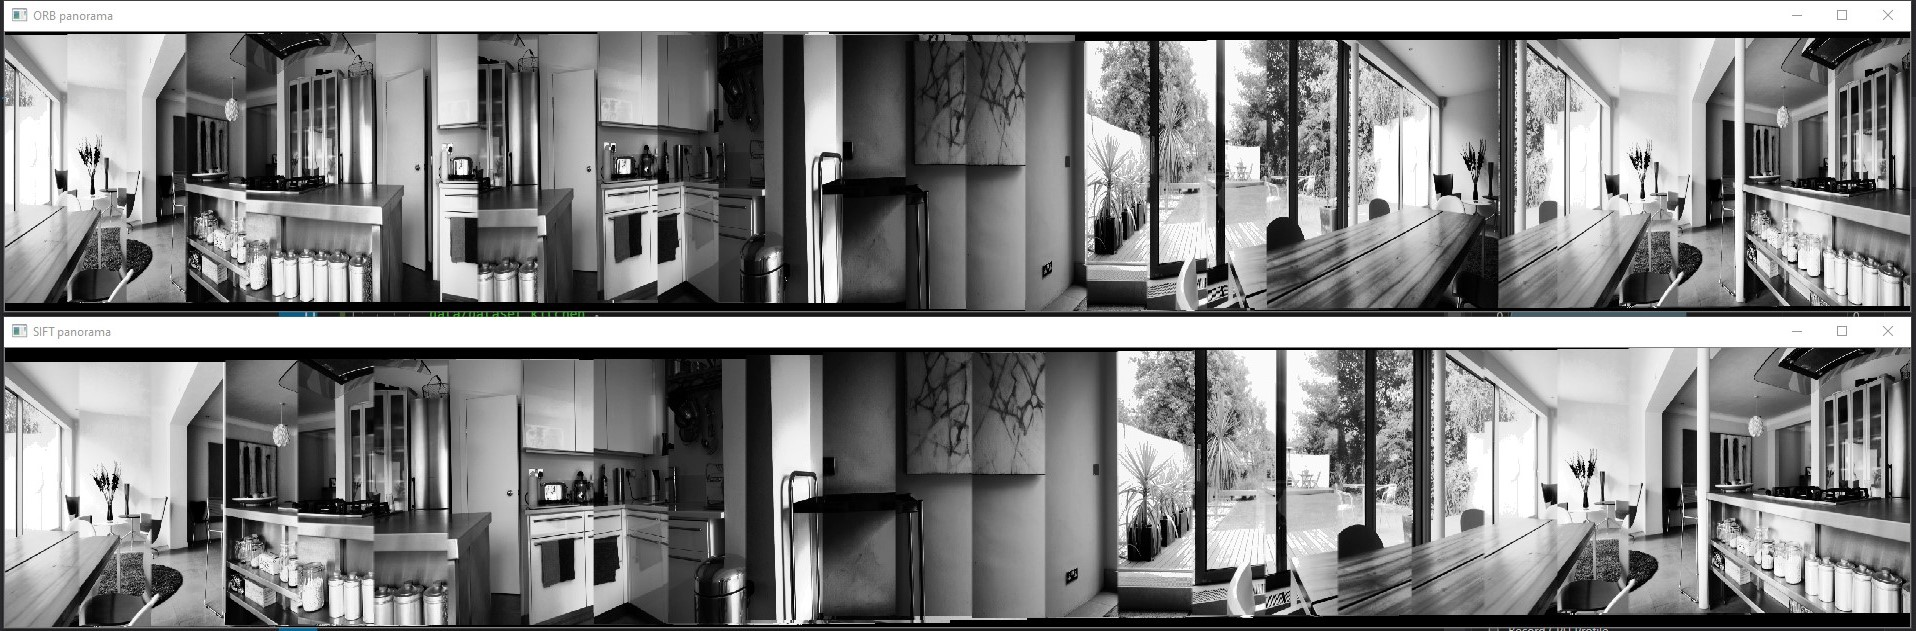
\includegraphics[width=1\textwidth]{images/kitchen}
\caption{\footnotesize{the Kitchen dataset provide an almost perfect result, apart from some illumination differences.}}
\label{img_kitchen}
\end{center}
\end{figure}

\begin{figure}[h]
\begin{center}
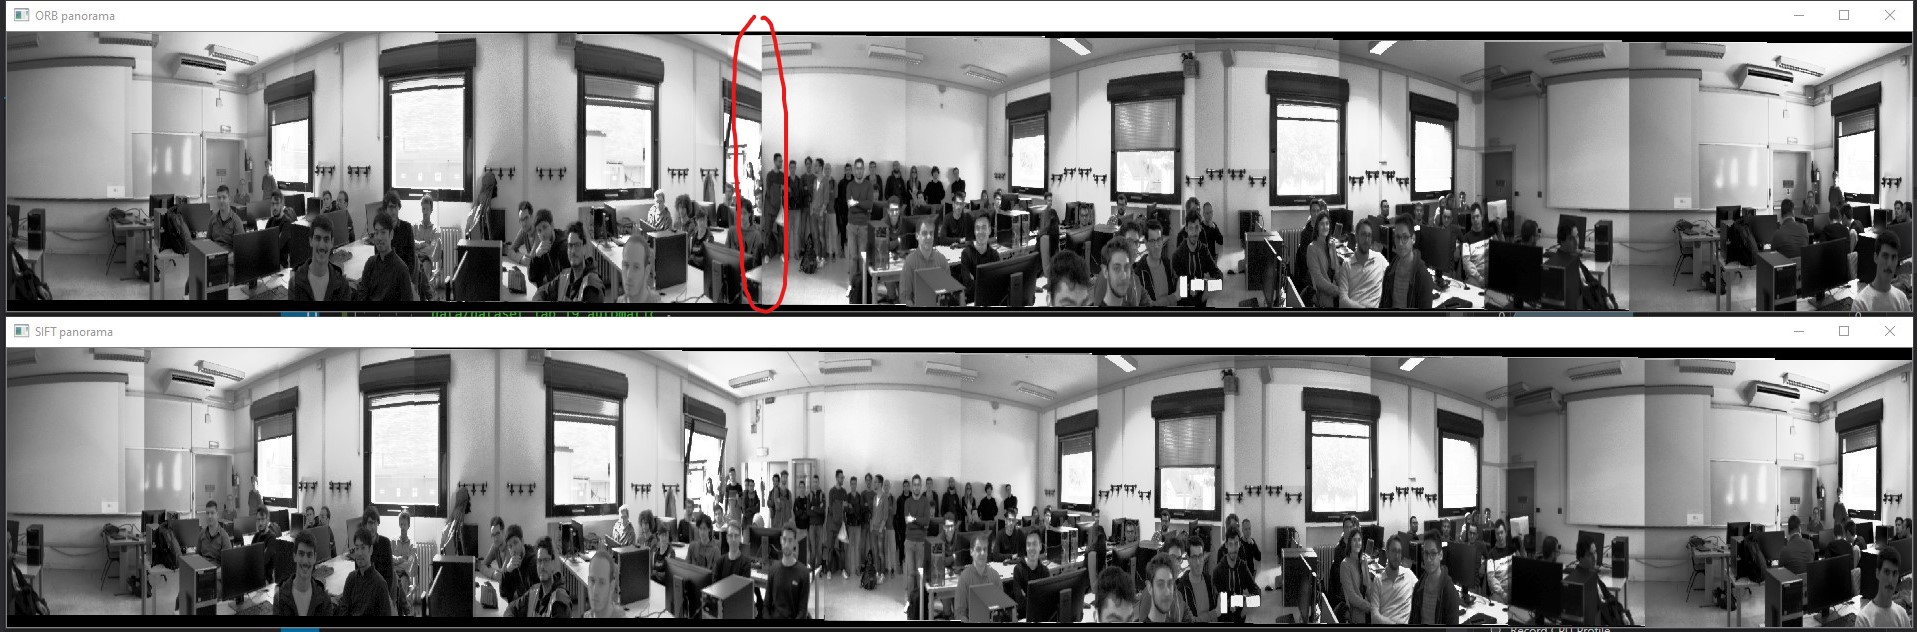
\includegraphics[width=1\textwidth]{images/lab_19_automatic}
\caption{\footnotesize{this is an example where ORB is not able to provide good enough features, as highlighted.}}
\label{img_lab_19_automatic}
\end{center}
\end{figure}

\end{document}